\documentclass[11pt]{jsarticle}

\usepackage{SPR}

\headerSPR
\begin{document}
	\titleSPR{\number\year}{\number\month}{\number\day}{D1}{吉田 皓太郎}
%%%%%%%%%%%%%%%%%%%%%%%%%%%%%%%%%%%%%%
	\articleSPRabst
		\begin{itemize}
			\item 定性的な機能を満たすカップの設計支援
		\end{itemize}
		
		
	\articleSPRobj
		\begin{enumerate}
			\item 定性的な要求を,最適化問題によって表現することで,数理処理が可能となる.
			\item 事例をベースとした機械学習を用いることで,ある程度の確かさが確保できると思われる.
		\end{enumerate}
%%%%%%%%%%%%%%%%%%%%%%%%%%%%%%%%%%%%%%
% 1.前回からのノルマ
	\articleSPRitemsone
		%\begin{enumerate}
		%	\item A
		%\end{enumerate}
		
		\tableofcontents
		
		
%%%%%%%%%%%%%%%%%%%%%%%%%%%%%%%%%%%%%%
%\begin{itemize}
%	\item 新規手法について
%	\item ISFAアウトライン
%\end{itemize}
%%%%%%%%%%%%%%%%%%%%%%%%%%%%%%%%%%%%%%
% 2.具体的な成果
	\articleSPRitemstwo
\renewcommand{\labelitemi}{$\blacktriangledown$}
%%%%%%%%%%%%%%%%%%%%%%%%%%%%%%%%%%%%%%
	\section{機械学習の手法について}
		\subsection{緒論}
			ブラジャーカップのユーザのニーズは様々であり,定量化できるものとそうでないものがある.例えば,身体にフィットするという機能は,という要求は身体形状とカップ形状との差分が一番小さくなればよい,という定量的な説明をすることができる.一方で定性的な要求もたくさん存在するが,その定性的な度合は様々で,「美しい」などいった個々の感情一つで評価が変わる項目もあるが,「寄せて上げる」など,定量的ではないにしても,ある程度共通の評価をすることができる項目もある.本研究では,そのようなある程度共通の評価を行うことができ,カップ形状が発現できる機能の一つである「寄せる」という機能に着目し,その要求を満たすようなカップ形状を設計支援する手法を構築する.
		\subsection{問題へのアプローチ}	
			設計者は,寄せてあげる機能を持つようなブラジャーカップの形状を経験的に知っているが,そのカップ形状との関連については述べていない.すなわち,その効用関数を決定する形状の特徴量は知っているわけではない.このような熟練者の経験と勘によって起こる問題に対し,機械学習によるアプローチが試みられており,一定の有用性が確かめられている.本研究でも,機械学習を用いたアプローチを行うことを考える.
		\subsection{機械学習の概要}
			機械学習は,一般にある入力パラメータ$ \bd{x} $に対しての出力値$ \bd{y} $が与えられた場合に,それらの相関を表現する$ \bd{y} = \bd{f} (\bd{x}) $の$ \bd{f} (\bd{x})  $を求めることを意味する.今回では,機能の発現$c = 0 or 1 $を出力とし,入力パラメータを,カップ形状の特徴量であるとする.このようにおけば,二つの関係を表す関数を得ることができると思われる.今回は,特定のワイヤー形状に対し,ある三次元データのカップ形状およびパターン形状における,設計者が判断した機能の発現状態を学習させることを考える.
		\subsection{カップのデータについて}
			今回は,簡略化のためにカップの接ぎラインがすでに与えられている場合について考える.曲線には二階微分性が確保されていれば,入力する形(B-spline,ベジエなど)は問わない.この曲線およびワイヤーデータから接ぎラインの曲線を決定する関数である物体標構の回転率ベクトルを導出する\footnote{この導出に関しては,M2からD1の間に出した論文や学会で発表している通りなので省略いたします.}.また,曲面データが求まることから,ここから体積を求める.体積については,一般に以下の式で求められるとする.
			\begin{equation}\label{eq:VolGeneralEq}
				V = \int_x \int_y z dxdy
			\end{equation}
			曲面の一般座標$ \bd{S}(s,t) $が以下の式で表されていることを利用する.
			\begin{equation}\label{eq:GeneralSurfaceEq}
				\bd{S}(s,t) = \bd{p}(s) + t \bd{d}_2(s)
			\end{equation}
			これを基にヤコビ変換をすると以下のように表される.
			\begin{equation}\label{eq:JacobiEq}
				dxdy = (\bd{S}_s \cdot \bd{e}_x \bd{S}_t \cdot \bd{e}_y - \bd{S}_s \cdot \bd{e}_y \bd{S}_t \cdot \bd{e}_x)dsdt 
			\end{equation}
			これらをカップの特徴量として,学習データに保存する.
		\subsection{データの識別}
			本研究では,あるバストの点群形状が与えられる場合を考える.カップを設計する際,バストとはある程度近いものを選定する必要がある.今回は,バストとカップとのデータの近さを定義するため,体積を考える.まずバスト体積$ V_b $を計算する.この体積を用いてある閾値$ \varepsilon $を用いて以下の条件によって,近いデータを識別する.
			\begin{equation}\label{eq:Divide}
				\frac{V-V_b}{V_b}<\varepsilon
			\end{equation}
		\subsection{事前学習データの作成}
			閾値によって集められたデータにおいて,回転率ベクトルは離散的な点集合で定義される曲線である.機械学習の際には,この曲線をいくつかのパラメータによって表現されるべきである.本研究では,画像解析分野でよく用いられるフーリエ展開を行い,その級数を記述する係数を用いて表現する.
			このパラメータと機能発現の出力をガウス過程のクラスタリングさせることで,未知の事後パラメータ入力に対してどれだけ機能が発現したかを求めることができる.この出力に対する目的関数を最大化(最小化)するように入力を求める方法は,ベイズ最適化と呼ばれ,分散と平均を用いて定義される獲得関数を最大化する最適化問題へと変換することで,目的関数が未知の形であっても,最適化を行うことができるようにする手法である.
		\subsection{本研究における最終目的と課題}
			本研究が達成する目的としては,機能の発現を満たしたブラジャーカップを設計することである.ただ,あくまで目標とするバストに近いものでなければならないため,バストとカップのフィット具合を表す関数$ f $\footnote{ISFA2020と同じ目的関数}も最小化されなければならない.また,カップに関する制約を考えると,可展面であることも考慮して,
			\begin{itemize}
				\item 可展開条件
				\item 終点座標の一致
			\end{itemize}
			など,様々な制約が考えられる.よって,まとめると以下のような最適化問題に帰結される.
			\begin{eqnarray}
				\mathrm{Minimize} &&\;\;f \\
				\mathrm{Maximize} &&\;\;c \\
				\mathrm{s.t.} &&\;\;h_j=0\;\;(j=0,\cdots n_c)
			\end{eqnarray}
			過去には,制約を加味したベイズ最適化なども提案されてきた\footnote{(BeyesianOptimization Constraints)で検索するといくつか論文が出てくる}が,事前学習データに制約も追加で学習させなければならないが,本研究で与える事前学習データは,その全てがすでにクリアされている状態で入力されるため,学習過程でパラメータによって影響されないと判断されてしまう問題がある.(あくまで統計処理に基づいているため)
			\subsection{問題点に対するアプローチ}
			本研究では,そのような問題に対して,事前学習させるタイミングで,パラメータを摂動させたときの制約の値を学習させることで,制約の平均や分散を定義できるようにすることを考える.このとき,どのように摂動させることが問題となる.ここで,フィット関数や制約が数理的に処理されるのに対し,機能発現が統計的に処理されることから,本研究では,機能発現関数の微小振動について考える.機能発現の事後パラメータ$ \bd{a}^* $における期待値は文献(GausssianProcessforMachineLearning)に挙げられるように,解析的に求めることが可能になっている.ある入力データのパラメータ$ \bd{a}_i $付近で,この関数を摂動展開してみる.
			\begin{equation}
				c = \Phi\left( \delta(\bd{a}_i+\Delta \bd{a})\right) = \Phi\left( \delta(\bd{a}_i)\right) + \frac{\partial \Phi(\bd{a}_i)}{\partial \bd{a}_i} \Delta \bd{a}
			\end{equation}
			詳しい$ \delta(\bd{a}^*) $は関連項目に記載する.(間に合わなければすみません.出展で書いてあるのでぜひ参考にしてみてください,英語文献ですが・・・)このとき,摂動因子を
			\begin{equation}\label{eq:FreEq}
				\eta_{i,j} = \min_j \frac{\partial\Phi(\bd{a}_{i})}{\partial a_{i,j}} 
			\end{equation}
			としておき,微小移動ベクトルを$ \bd{d}_{j} = \nu \bd{e}_j$とおく.ここで$ \bd{e}_j $は$ j $次元目の単位ベクトルを表す.そして,$ \bd{a}^*_i = \bd{a}_i+\eta_{i,j} \bd{d}_j $として,フィット関数と制約条件を再計算することで,クラスタリングに関する学習データの影響を少なくさせつつ制約の値のばらつきを生じさせることができる.これを用いてフィット関数および制約条件を再学習したデータを用いて,制約付きベイズ最適化を行うことができる(はず).以上をまとめて,システムのフロチャートに記すと以下のように記述される.
			\begin{figure}[h!]
				\centering
				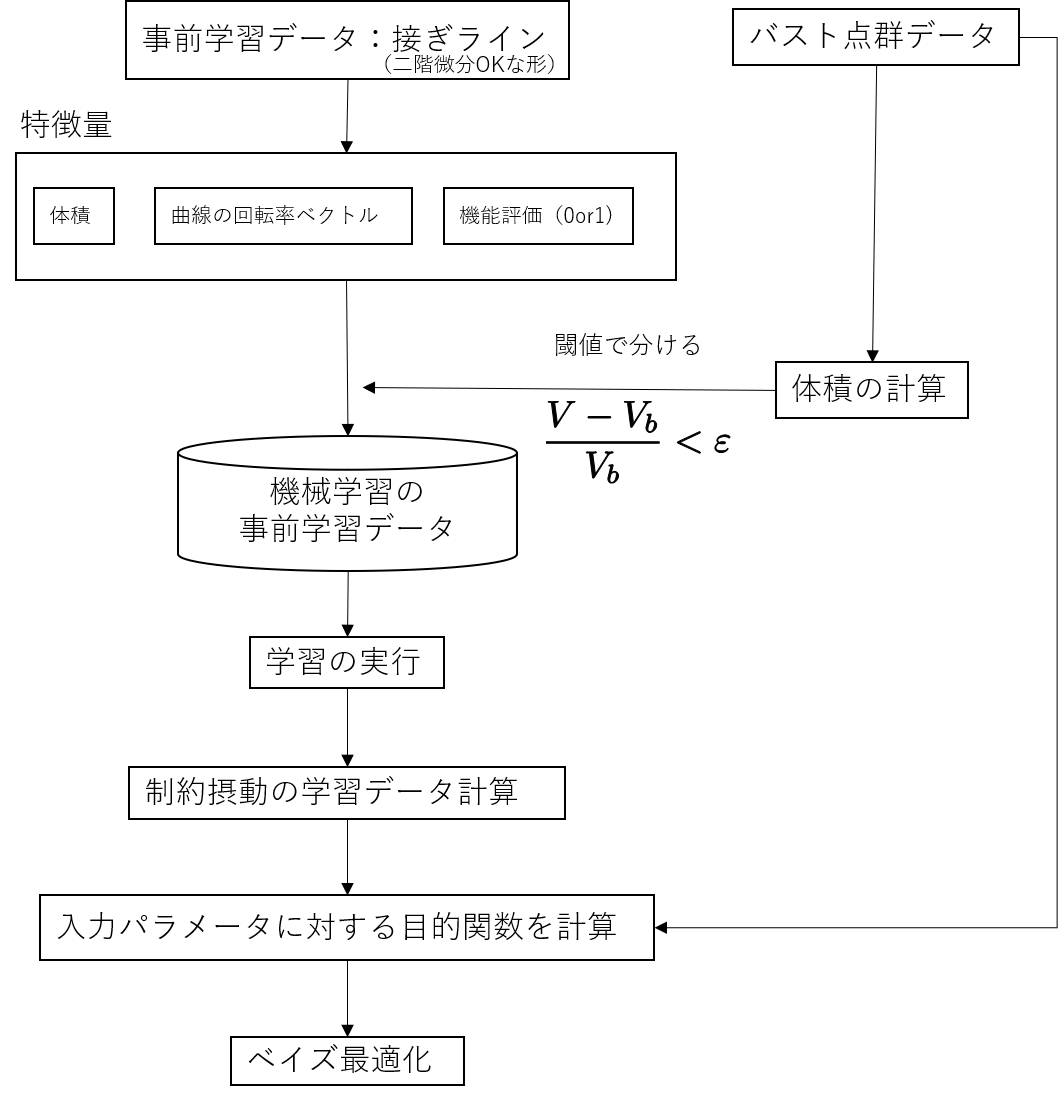
\includegraphics[scale=0.45]{./Figure/OptFlow.png}
				\caption{システムの概念図}
			\end{figure}
	\section{布物性のシミュレーションについて}
		以下に示す項目が,自分の中で少し疑問に感じたので共有しておきます.もしご意見あれば頂けると幸いです.
		\begin{itemize}
			\item 【目的】布の伸びと紙模型との関連性が分からなかった→これでいいのか
			\item 既存の着装シミュレーションとどういう部分で違いをもたせるべきなのか
			\item この変形シミュレーションは何が難しいのか
		\end{itemize}
	\section{その他}
		\begin{itemize}
			\item ISFA2020は一度目を通したのち,直接投稿してよろしいですか?(Copyrightは提出済)
			\item 繊維機械学会は請求書を保存しておけばいいですか?
			\item 学外PCから,リモートとかダメですかね...?
		\end{itemize}
	
	\section{ガウス過程について}
ある入力パラメータ$ \bd{x} $と,出力パラメータ$ \bd{y} $が,正規分布$ N(\bd{\mu},\bd{\Sigma}) $に従うとき,出力がガウス過程に従うという.このガウス過程は,ニューラルネットワークの中間ノード数無限の極限としても知られる(Neal,1996).
	\subsection{ガウス過程の概要}
		入力パラメータ$ \bd{x} $と,出力パラメータ$ \bd{y} $について,その関係$ \bd{y} = \bd{f}(\bd{x})$を求めることを考える.単純な手法としては,以下のように,基底関数$ \bd{\Phi}(\bd{x}) $を用いて,以下のような重み付きの線形和で表し,この重みを最小二乗法などで求める手法である.
		\begin{equation}\label{eq:Ritz_ppoi}
			\bd{y} = \bd{\Phi}\bd{w}
		\end{equation}
		この基底関数には,以下のような動径基底関数を用いればよいとされ,この方法は,動径基底関数回帰と呼ばれる.
		\begin{equation}\label{eq:phieq}
			\phi_i = \{\bd{\Phi}\}_i = \exp\left(-\frac{(x-\mu_h)^2}{\sigma^2}\right)
		\end{equation}
		しかし,この手法は$ \mu_h $を,入力の定義域上になるべく多く配置させる必要があり,$ \bd{x} $の次元に対して指数的に増加する\footnote{次元の呪いとも呼ばれる}ため,現実的に解くのは非常に難しいとされる.
		
		そこで,$ \bd{w} $があるガウス分布$ N(0,\lambda^2\bd{I}) $に従うとするときについて考える.このとき,$ \bd{y} = \bd{\Phi}\bd{w} $もまた,ガウス分布に従う.このとき,モデルの期待値および分散は以下のように求められる.
		\begin{eqnarray}\label{eq:VarandAvg}
			E[\bd{y}] &=& E[\bd{\Phi}\bd{w}] = \bd{\Phi}E[\bd{w}]=0\\
			\Sigma &=& E[\bd{y}\bd{y}^T]-	E[\bd{y}]E[\bd{y}^T] = \lambda^2\bd{\Phi}\bd{\Phi}^T
		\end{eqnarray}
		よって,$ \bd{y} $はガウス分布$ N(\bd{0},\lambda^2\bd{\Phi}\bd{\Phi}^T) $に従う.$ \bd{K} =  \lambda^2\bd{\Phi}\bd{\Phi}^T$と置けば,$ \bd{K} $が求めれば,$ \bd{y} $のガウス分布を求めることができる.
		この$ \bd{K} $は,グラム行列,またはカーネル行列と呼ばれ,その行列が下記の条件を満たすように設計されなければならない.
		\begin{itemize}
			\item 逆行列の存在を保証する.
			\item 正定値を持つ.
			\item 固有値が全て正である
		\end{itemize}
		カーネル行列の各成分を示すカーネル関数として代表的なものは,以下で示すRBFがある.なお,$ \bd{\theta} = [\theta_1,\theta_2] $は,ハイパーパラメータと呼ばれる.
		\begin{equation}\label{eq:Kernel}
			k(\bd{x}_i,\bd{x}_j) = \theta_1 \exp\left(- \frac{|\bd{x}_i-\bd{x}_j|^2}{2 \theta_2^2}\right)
		\end{equation}
		このモデルを用いて,ある事前学習パラメータ$ \bd{X}=[\bd{x}_1,\bd{x}_2,\cdots,\bd{x}_n] $に対し,$ \bd{Y}=[y_1,y_2,\cdots,y_n] $という出力が得られている場合において,ある入力パラメータ$ \bd{x}_* $に対する$ y_* $は事後確率の期待値として表される.
		\begin{equation}
			y_* = \bd{k}_* \bd{K}^{-1} \bd{Y}
		\end{equation}
		ただし,$ \bd{k}_* = \{k(\bd{x}_*,\bd{x}_i)\}_{i=1}^{n} $である.
		
		ハイパーパラメータの定め方について述べる.このとき,確率関数の対数をとった尤度関数は以下のように表される.
		\begin{equation}\label{eq:Suudo}
			\log(p) = -\log|\bd{K}_{\theta}| - \bd{y}^T \bd{K}_{\theta}^{-1} \bd{y}+C
		\end{equation}
		ただし,ハイパーパラメータに無関係な定数をまとめて$ C $とおいている.一般にはこの尤度関数を最大化するような最適化問題を解くことによって,パラメータを得る.この最適化問題は解析的に微分を求めることができるため,勾配法を用いて解くケースが多い.
	\subsection{クラスタリングについて}
		出力として二値的な値を取る場合,出力の値を近似的に$ y = \sigma(\bd{x}) $と表す,ただし,$ \sigma(\bd{x}) $はシグモイド関数である.このとき,事後確率の出力は少し複雑となり,以下のように表される.
		\begin{equation}\label{eq:y_*=1}
			q = \Psi\left( \frac{\bd{k}_*^T \tilde{\bd{K}}^{-1} \tilde{\bd{\mu}}}{\sqrt{1+k(\bd{x}_*,\bd{x}_*)-\bd{k}_*^T \tilde{\bd{K}}^{-1} \bd{k}_*}} \right)
		\end{equation}
		ここで,$ \Psi $は累積分布関数を表す.また,$ \tilde{\bd{K}} $や$ \tilde{\bd{\mu}} $は特定のアルゴリズムを用いて求められる(事後学習のデータを用いることなく)が,ここでは省略する.
	\subsection{ベイズ最適化について}
	ベイズ最適化は,ガウス過程を応用する形になっており,ある目的関数$ f(\bd{x}) $を最小化するような$ \bd{x} $を求める手法である.ここでは,ある学習データが与えられる場合について考える(学習データがない場合は,一様に初期解を生成する手法があるらしい?).このとき,この最適化問題は,事後学習における平均および分散の関数で定める適当な関数の最適化問題に変換でき,関数を明示的に与える必要がないのが,ベイズ最適化の特徴である.この目的関数の定め方は色々あるが,ポピュラーなものとしてはEIがある.
	\begin{equation}\label{eq:Zeq}
		Z = \frac{\mu - f^+ -\xi}{\sigma}
	\end{equation}
	\begin{equation}
		a_{EI} = (\mu - f^+ -\xi)\Psi(Z) + \sigma \psi(Z)
	\end{equation}
	ただし,$ \psi(x) \sim N(0,1)$の正規分布関数である.
	\newpage
\vspace{10cm}
%%%%%%%%%%%%%%%%%%%%%%%%%%%%%%%%%%%%%%
% 3.達成できなかったこととその問題点
	%\articleSPRthree
%%%%%%%%%%%%%%%%%%%%%%%%%%%%%%%%%%%%%%

\vspace{14cm}
%%%%%%%%%%%%%%%%%%%%%%%%%%%%%%%%%%%%%%
	\articleSPRfour
	\articleSPRfive
\end{document}
